\subsection{Driven sweet spots}
\label{subsec:ssconditiondiscussion}
\begin{figure*}[t]
    \centering
    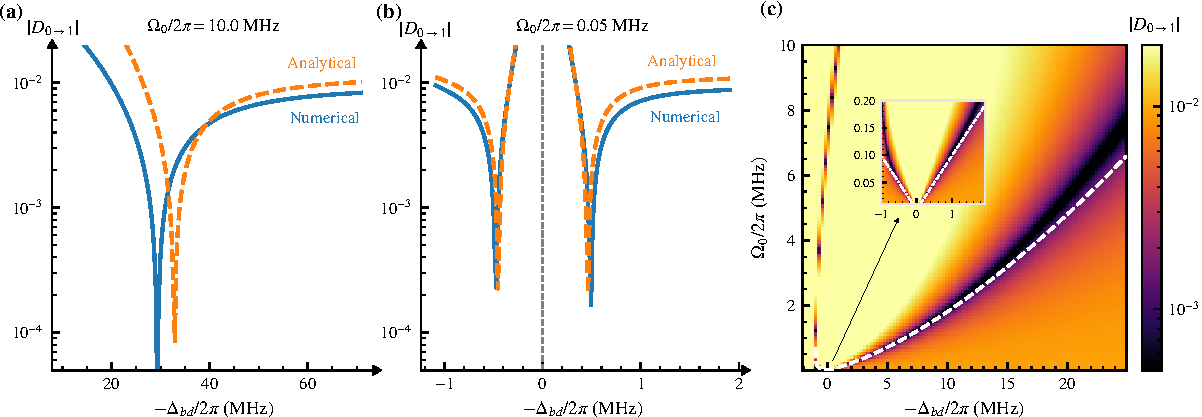
\includegraphics[width=\textwidth]{Sec 2/compare.pdf}
    \caption[Drive-induced flux sweet spots, defined by \(D_{0\rightarrow 1}=0\).]{Drive-induced flux sweet spots, defined by \(D_{0\rightarrow 1}=0\).
(a) Unselective regime at \(\Omega_0/2\pi=10~\mathrm{MHz}\), showing a single sweet spot.
(b) Selective regime at \(\Omega_0/2\pi=0.05~\mathrm{MHz}\), showing two symmetric sweet spots about the effective resonance.
(c) Two-dimensional map of \(D_{0\rightarrow 1}\) versus drive amplitude \(\Omega_0\) and detuning \(\Delta_{bd}\); Dashed curves denote analytical sweet-spot conditions from Eqs.~\eqref{perturbation energy} and \eqref{eq:Dm_selective} for the main panel and the inset, respectively.}
\label{fig:compare}
\end{figure*}

FTT frequency fluctuations $\delta\omega_b(t)$ are converted into cavity-frequency fluctuations $\delta\bar{\omega}_c(t)$ through the Lamb shift, producing cavity dephasing. This dephasing channel can be suppressed by driving the FTT [Fig.~\ref{fig:device}(a)], which induces a photon-number--dependent energy shift that can be tuned to cancel the Lamb-shift fluctuations.

In the frame rotating at the drive frequency $\omega_d$, the driven dispersive Hamiltonian reads
\begin{equation}
\label{eq:H_R_floquet}
H_R =
\Delta_{bd}\, b^\dagger b
+ \frac{K}{2}\, b^{\dagger 2} b^{2}
+ \overline{\omega}_c\, c^\dagger c
+ \chi\, b^\dagger b\, c^\dagger c
+ \Omega_0\, ( b + b^\dagger ),
\end{equation}
where $\Delta_{bd}=\bar{\omega}_b-\omega_d$ is the FTT--drive detuning. The drive couples $|g,m\rangle$ and $|e,m\rangle$ at fixed cavity photon number $m$, producing level repulsion that lowers the energy of $|g,m\rangle$. The dispersive interaction offsets the detuning by $m\chi$, so the relevant detuning is $\Delta_m \equiv \Delta_{bd}+m\chi$ and the drive-induced energy shift becomes photon-number dependent. Examples for $m=0,1$ are shown in Fig.~\ref{fig:device}(c), and this $m$-dependent shift can be tuned to cancel fluctuations of the static Lamb shift [Fig.~\ref{fig:device}(d)].

An analytic expression follows in the weak-drive regime, assuming (i) $\Omega_0 \ll \min_m|\Delta_m|$ over the photon numbers of interest, so that the drive does not strongly hybridize $|g,m\rangle$ and $|e,m\rangle$, and (ii) $|\Omega_0|\ll |K+2\Delta_{bd}|$, so that hybridization with the state $|f,m\rangle$, remains weak. Under these conditions, a Schrieffer--Wolff transformation (Appendix~\ref{SWT}) diagonalizes $H_R$. Retaining terms up to $\mathcal{O}(\Omega_0^2/\Delta_m^2)$ and projecting onto the $\{|g,m\rangle,|e,m\rangle\}$ subspace gives
\begin{equation}
\label{eq:mainHd_two_level}
\begin{aligned}
H_d =\;&
\widetilde{\Delta}_{bd}\,\sigma^+\sigma^-
+\bar\omega_c\,c^\dagger c
-\sum_m \frac{\Omega_0^2}{\Delta_m}\,|m\rangle\langle m|
\\
&+\sigma^+\sigma^-\!\left[
\chi\,c^\dagger c
+\sum_m \frac{2\Omega_0^2}{\Delta_m}\,|m\rangle\langle m|
\right],
\end{aligned}
\end{equation}
where $\sigma^+\sigma^- \equiv |e\rangle\langle e|$ and $|m\rangle$ denotes a cavity Fock state. The drive renormalizes the FTT detuning, $\widetilde{\Delta}_{bd}\equiv \Delta_{bd}-\Omega_0^2/K$, and generates an $m$-dependent shift of the cavity transition frequency together with an additional Stark shift. The essential point is that this drive-induced shift can be tuned to cancel the flux-sensitive static Lamb shift, thereby creating a driven sweet spot.

To quantify the resulting cavity-frequency fluctuation, we define the net cavity
transition frequency between adjacent cavity levels as
\begin{equation}
\label{perturbation energy}
\widetilde{\omega}_{c,m\rightarrow m+1}=\bar{\omega}_c-\Omega_0^2/\Delta_{m+1}+\Omega_0^2/\Delta_m.
\end{equation}
We use a bar for Lamb-shifted frequencies and a tilde for drive-renormalized transition frequencies.
FTT frequency fluctuation $\delta\omega_b(t)$ then induces
\begin{equation}
\delta\widetilde{\omega}_{c,m\rightarrow m+1}(t)= D_{m\rightarrow m+1}\,\delta\omega_b(t)
\end{equation}
where $D_{m\rightarrow m+1}\equiv \frac{\partial \widetilde{\omega}_{c,m\rightarrow m+1}}{\partial \omega_b}$ is the susceptibility of the net cavity frequency to FTT-frequency fluctuation.
It has two contributions: a bare term inherited from the Lamb-shift dependence
$\bar{\omega}_c(\omega_b)$, and a drive-induced term from the dressing shift through $\Delta_m=\Delta_{bd}+m\chi$. A sweet spot occurs when these two terms cancel. Specifically, the physics of the cancellation differs in two regimes.


\paragraph{Unselective Regime.}
In this regime, the drive detuning \(\Delta_{m^\ast}\equiv \Delta_{bd}+m^\ast\chi\) satisfies \( |\Delta_{m^\ast}|\gg|\chi| \), so the drive couples
\(\ket{g,m^\ast}\leftrightarrow\ket{e,m^\ast}\) and neighboring photon-number pairs with comparable strength.
As a result, the effective cavity nonlinearity near \(m^\ast\) is suppressed.
For \(m^\ast=0\), expanding the denominators
\(\Delta_m^{-1}=(\Delta_{bd}+m\chi)^{-1}\) to leading order in \(|\chi/\Delta_{bd}|\) yields the approximate effective Hamiltonian
\begin{equation}
\label{eq:Hd_far_detuned}
H_d \approx
\widetilde{\Delta}_{bd}\,\sigma^+\sigma^-
+\widetilde{\omega}_{c,0\rightarrow 1}\,c^\dagger c
+\chi\left(1-\frac{2\Omega_0^2}{\Delta_{bd}^2}\right)\sigma^+\sigma^-\,c^\dagger c ,
\end{equation}
up to constant energy offsets, where
\begin{equation}
\widetilde{\omega}_{c,0\rightarrow 1}=\bar{\omega}_c+\frac{\Omega_0^2\chi}{\Delta_{bd}^2}.
\end{equation}
The corresponding susceptibility of the net cavity frequency is
\begin{equation}
\label{eq:D01_unselective}
D_{0 \rightarrow 1}
\approx \frac{g^2}{\Delta_{bc}^2}\left[1-\frac{4\Omega_0^2K}{\Delta_{bd}^3}\right].
\end{equation}
The far-detuned sweet spot is therefore set by \(D_{0 \rightarrow 1}=0\), which gives the single solution
\begin{equation}
\label{eq:ss_unselective}
\Delta_{bd}=\sqrt[3]{4\Omega_0^2K}.
\end{equation}

This prediction is confirmed by Fig.~\ref{fig:compare}(b).
Because the rotating-frame spectrum of \(H_R\) approximates the Floquet quasienergies (defined modulo \(\omega_d\); see App.~\ref{app:floquet}), the analytical susceptibility is compared against a Floquet calculation using the full-model Hamiltonian (App.~\ref{app:numerics}).
For \(\Omega_0/2\pi=10~\mathrm{MHz}\), \(D_{0 \rightarrow 1}\) approaches the bare Lamb-shift value \(g^2/\Delta_{bc}^2\approx0.01\) when the drive is far detuned from the FTT frequency \(\bar{\omega}_b\).
As \(\omega_d\) is tuned toward \(\bar{\omega}_b\), a single sweet spot appears on the \(\omega_d>\bar{\omega}_b\) side, consistent with the negative anharmonicity of the FTT.
The characteristic detuning is consistent with Eq.~\eqref{eq:ss_unselective}, which predicts \(\Delta_{bd}/2\pi\sim -34~\mathrm{MHz}\) for \(K/2\pi\approx-0.1~\mathrm{GHz}\) used here.
The residual offset between the analytical and numerical dip positions at this drive strength arises because higher-order corrections to the Hamiltonian Eq.~\eqref{eq:mainHd_two_level} become non-negligible.
Closer to resonance, \(D_{0 \rightarrow 1}\) rises again as the drive-induced energy shift dominates the susceptibility.

\paragraph{Selective Regime.}
In this regime, the drive is closest to resonance for a particular photon number \(m^\ast\), so that \(|\Delta_{m^\ast}|\ll \chi\).
Consequently, only the hybridization between \(\ket{g,m^\ast}\) and \(\ket{e,m^\ast}\) contributes appreciably to the cavity frequency, giving
\begin{equation}
\widetilde{\omega}_{c,m^\ast\rightarrow m^\ast+1}
\approx
\bar{\omega}_c+\frac{\Omega_0^2}{\Delta_{m^\ast}}.
\end{equation}
Differentiating with respect to \(\omega_b\) yields
\begin{equation}
\label{eq:Dm_selective}
D_{m^\ast}
\approx
\frac{g^2}{\Delta_{bc}^2}
-\frac{\Omega_0^2}{\Delta_{m^\ast}^2}.
\end{equation}
Setting \(D_{m^\ast}=0\) gives the sweet-spot condition
\begin{equation}
\label{eq:weak_drive_sweetspot}
\Delta_{m^\ast}=\pm \left|\frac{\Delta_{bc}}{g}\Omega_0\right|
\Longleftrightarrow
\Delta_{bd}=\pm \left|\frac{\Delta_{bc}}{g}\Omega_0\right|-m^\ast\chi .
\end{equation}

This prediction is confirmed by Fig.~\ref{fig:compare}(a), where two sweet spots appear as symmetric dips on either side of the resonance.
Their characteristic detuning is consistent with Eq.~\eqref{eq:weak_drive_sweetspot}, which predicts
\(|\Delta_{bd}|\sim (|\Delta_{bc}|/g)\Omega_0\approx 0.5~\mathrm{MHz}\) for the parameters used here (\(g/|\Delta_{bc}|\simeq 0.1\)).
Overall, the agreement between the analytics and exact numerics shows that in the selective regime a low-power drive cancels the bare Lamb-shift susceptibility.

% \footnote{For $m^*>0$, at the sweet spot where $D_{m^*}=0$, the neighboring susceptibility remains
% $D_{m^*-1}\approx 2g^2/\Delta_{bc}^2$, implying that the dephasing between the $|m^*-1\rangle, |m^*\rangle$ states is approximately doubled relative to the undriven rate.}.

\paragraph{Sweet-Spot Map and Regime Crossover.}
Fig.~\ref{fig:compare}(c) shows \(D_{0\rightarrow 1}\) as a function of drive amplitude \(\Omega_0\) and detuning \(\Delta_{bd}\). The key point is that the selective and unselective sweet spots are not distinct phenomena, but rather different parts of a continuous contour defined by \(D_{0\rightarrow 1}=0\). At small \(\Omega_0\), the selective-regime condition in Eq.~\eqref{eq:weak_drive_sweetspot} predicts the linear scaling \(|\Delta_{bd}| \propto \Omega_0\), visible as two symmetric sweet spots on either side of the effective resonance. As \(\Omega_0\) increases, the inner branch, closer to resonance and at smaller \(|\Delta_{bd}|\), enters a nonperturbative regime in which the weak-drive approximation underlying Eq.~\eqref{eq:mainHd_two_level} no longer applies. The remaining perturbative branch then crosses over toward the unselective regime and approaches the cubic scaling predicted by Eq.~\eqref{eq:ss_unselective}. At still larger \(\Omega_0\), the Stark-shift contribution broadens the detuning range over which \(D_{0\rightarrow 1}\approx 0\), improving robustness against flux noise by maintaining susceptibility cancellation over a wider range of fluctuations, albeit closer to the limits of perturbation theory. Higher-order drive effects generate additional sweet spots; see App.~\ref{higher-order app}. The same mechanism is not restricted to the FTT and is illustrated for a SNAIL-based circuit in App.~\ref{snail}. Finally, although the sweet-spot condition does not in general suppress sensitivity to drive-amplitude noise, for AWG noise levels typical of experiments the associated dephasing is negligible, see App.~\ref{app:amplitude_noise}.





